\documentclass[twoside, 12pt]{article}
\usepackage{amssymb, amsmath, mathrsfs, amsthm} %for math environments
\usepackage{graphicx} %for figures
\usepackage{color} %mostly for listings package, also hyperlinks
\usepackage[top=2cm, bottom=2cm, left=2cm, right=2cm]{geometry} %page geometries
\usepackage{float, caption} %for figure formatting
\usepackage{listings} %to show notable code
\usepackage{hyperref} %hyperlinks
\usepackage{siunitx} %For units
\hypersetup{
    colorlinks=true,
    linkcolor=blue,
    filecolor=magenta,
    urlcolor=cyan,
}
\urlstyle{same}



\definecolor{codegreen}{rgb}{0,0.6,0}
\definecolor{codegray}{rgb}{0.5,0.5,0.5}
\definecolor{codepurple}{rgb}{0.58,0,0.82}
\definecolor{backcolour}{rgb}{0.95,0.95,0.92}

\lstdefinestyle{mystyle}{
    backgroundcolor=\color{backcolour},
    commentstyle=\color{codegreen},
    keywordstyle=\color{magenta},
    numberstyle=\tiny\color{codegray},
    stringstyle=\color{codepurple},
    basicstyle=\footnotesize,
    breakatwhitespace=false,
    breaklines=true,
    captionpos=b,
    keepspaces=true,
    numbers=left,
    numbersep=5pt,
    showspaces=false,
    showstringspaces=false,
    showtabs=false,
    tabsize=2
}

\definecolor{lightgray}{rgb}{.9,.9,.9}
\definecolor{darkgray}{rgb}{.4,.4,.4}
\definecolor{purple}{rgb}{0.65, 0.12, 0.82}
% Javascript not currently defined in listing package
\lstdefinelanguage{JavaScript}{
  keywords={break, case, catch, continue, debugger, default, delete, do, else, false, finally, for, function, if, in, instanceof, new, null, return, switch, this, throw, true, try, typeof, var, void, while, with},
  morecomment=[l]{//},
  morecomment=[s]{/*}{*/},
  morestring=[b]',
  morestring=[b]",
  ndkeywords={class, export, boolean, throw, implements, import, this},
  keywordstyle=\color{blue}\bfseries,
  ndkeywordstyle=\color{darkgray}\bfseries,
  identifierstyle=\color{black},
  commentstyle=\color{purple}\ttfamily,
  stringstyle=\color{red}\ttfamily,
  sensitive=true
}

\lstset{
   language=JavaScript,
   backgroundcolor=\color{lightgray},
   extendedchars=true,
   basicstyle=\footnotesize\ttfamily,
   showstringspaces=false,
   showspaces=false,
   numbers=left,
   numberstyle=\footnotesize,
   numbersep=9pt,
   tabsize=2,
   breaklines=true,
   showtabs=false,
   captionpos=b
}
%redefine Matlab styling
\lstset{language=Matlab,%
    %basicstyle=\color{red},
    breaklines=true,%
    morekeywords={matlab2tikz},
    keywordstyle=\color{blue},%
    morekeywords=[2]{1}, keywordstyle=[2]{\color{black}},
    identifierstyle=\color{black},%
    stringstyle=\color{mylilas},
    commentstyle=\color{mygreen},%
    showstringspaces=false,%without this there will be a symbol in the places where there is a space
    numbers=left,%
    numberstyle={\tiny \color{black}},% size of the numbers
    numbersep=9pt, % this defines how far the numbers are from the text
    emph=[1]{for,end,break},emphstyle=[1]\color{red}, %some words to emphasise
    %emph=[2]{word1,word2}, emphstyle=[2]{style},
}

\lstset{style=mystyle}
\graphicspath{{Images/}} %Images path set to folder in this directory
\lstset{inputpath=Input/} %Code and input path

%Math environoments
%TODO: add pseudo code packages
\theoremstyle{plain}
\newtheorem{theorem}{Theorem}
\newtheorem{lemma}{Lemma}
\newtheorem{definition}{Definition}
\newtheorem{corollary}[theorem]{Corollary}
\newtheorem{case}{Case}
\newtheorem{subcase}{Subcase}[case]
\newtheorem{claim}{Claim}
\newtheorem{subclaim}{Subclaim}[claim]
\newtheorem{fact}{Fact}
\newtheorem{problem}{Problem}
\newtheorem{proposition}{Proposition}
\newtheorem{constr}{Construction}
\newtheorem{question}{Question}
\newtheorem{algo}{Algorithm}
\newtheorem{conjecture}{Conjecture}
\renewcommand{\qedsymbol}{\sc q.e.d}
\newtheorem{remark}{Remark}

\date{} %Comment line to display current date

\linespread{1.5} %line spacing
\usepackage[nottoc]{tocbibind}

%%%%%%%%%%%%%%%%%%%%%%%%%%%%%%%%%%%%%%%%%%%%%%%%%%%%%%%%%%%%%%%%%%%%%%%%%%%%%%%%%%%%%%%%%%
% Formatting: careful with code separation, line skips result in new paragraphs
%
%%%%%%%%%%%%%%%%%%%%%%%%%%%%%%%%%%%%%%%%%%%%%%%%%%%%%%%%%%%%%%%%%%%%%%%%%%%%%%%%%%%%%%%%%%
\begin{document}
\title{EEG and Chaotic Time Series Analysis}
%\author{Add Contributors here}
\maketitle
\tableofcontents
\newpage
\begin{abstract}
How do we build a prosthetic limb that moves according to the thoughts of a wearer? Likewise, how do we communicate instructions to a computer using thoughts alone? Both questions are apart of the developing field of Brain-Computer Interfacing (BCI).

Electroencephalography (EEG) is one of the leading and affordable types of analysis of brain activity. We utilize a number of existing methods to filter and express these data. Furthermore, we illustrate approaches towards the categorization and prediction of these data through Artificial Neural Networks (ANNs). Finally, we implement a Nonlinear Autoregressive Exogenous (NARX) model for this prediction, and analyze the dynamics of the system.
\end{abstract}

\section{Introduction}
The human brain is an intricate and interwoven network of communicating cells, structures, and substructures. As such, understanding and interpreting information from this network is a primary research focus of many dedicated professionals. We aim to synthesize and present current understandings as succinctly as possible, for focus on how they may be utilized. To begin, we must define our operating principals.
\subsection{Electroencephalography (EEG)}
Traditionally, \textit{Electroencephalography} is the measurement of neuronal function given by the \textit{ionic gradient} of neuronal membranes \cite{tatum_handbook_2013}; typically given in microvolts and amplified for analysis. Electrical potentials are determined by individual \textit{neurons} consisting of four main parts: the \textit{Dendrites} or signal receptors, \textit{Soma} - main body of the cell, \textit{Axon} - for relaying signals, and the \textit{Terminal Bouton} - for transmitting signals via the synaptic gap. For the purpose of brevity, signals can be interpreted as either \textit{Excitatory Postsynaptic Potentials} (ESP) or \textit{Inhibitory Postsynaptic Potentials} (ISP), based on the influx of either sodium or potassium ions, respectively.
\begin{figure}[ht]
  \centering
  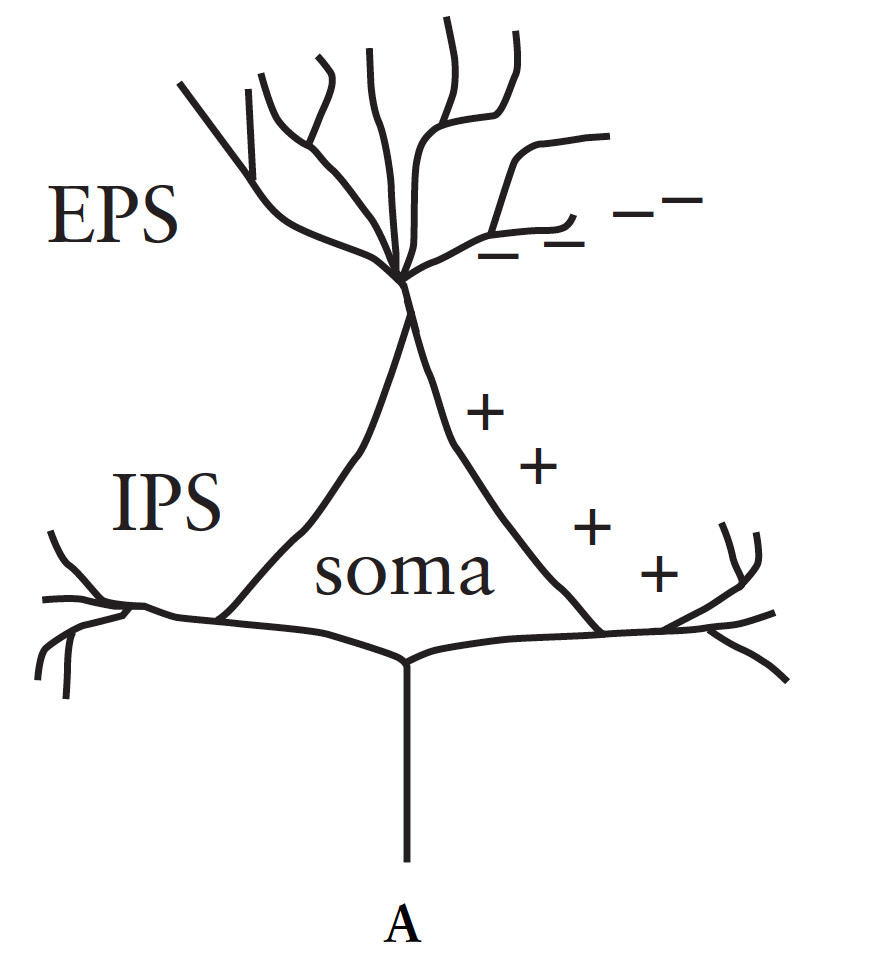
\includegraphics[width=2in]{Neuron.png}
  \caption{Neuron with inhibitory and excitatory signals - (where a is the axon)}
  \label{fig:neuron}
\end{figure}
The dendrites of the neuron receive both excitatory and inhibitory signals from adjacent neurons, which diffuse across the soma and trigger an \textit{action potential} based on the either positive or negative concentration of ions in the cell. This results in the propagation of signals across the axon, resulting in a consequent signal released by the terminal bouton into the synaptic gap. These events, known as \textit{synaptic potentials} are ultimately what are being measured by an EEG device.

We used the \href{http://docs.openbci.com/Headware/01-Ultracortex-Mark-IV}{OpenBCI Ultracortex Mark IV} headset for its open source design, 8 channels, and modifiable 3D-printed apparatus. The controlling Cyton board links via bluetooth interface with the OpenBCI USB Dongle, although the hardware allows for an insertable SD card for writing the data. The board samples at $\SI{250}{\hertz}$, which can be modified in the Cyton's Arduino firmware. Likewise, the scale factor of the received data is given as $\SI{0.02235}{\micro\volt}$, which is modifiable given the gain (default set to maximum) in the firmware or with live connection through development drivers such as the Python-MNE.
\subsection{Artificial Neural Networks (ANNs)}
%change wording of the first sentence
An \textit{Artificial Neural Network} is an information processing system based on the same principles as biological networks like the brain \cite{rudolf_computational_nodate}. The consist of a set of \textit{perceptrons} which work concurrently given activations on directed connections with each other. Much like neurons, the perceptrons send both excitatory and inhibitory signals, which influence the subsequent layers.

Formally, we express the neural network using a \textit{directed graph}.
\begin{definition}
\normalfont A \textit{Directed Graph}, $G$, consists of a set of \textit{vertices}, $V(G)$, and \textit{edges} ,$E(G)$. A \textit{directed edge} or \textit{arc}, $e = (u,v)\in E(G)$ represents a connection from the vertex $u$ to the vertex $v$. We define the \textit{predecessors} of $u$, $\textit{pred}(u)$, as $\left\{v\in V(G)\vert (v,u)\in V(G)\right\}$, and the \textit{succesors} of $u$, $\textit{succ}(u)$, as $\left\{v\in V(G)\vert (u,v)\in V(G)\right\}$.
\end{definition}
\begin{figure}[ht]
  \centering
  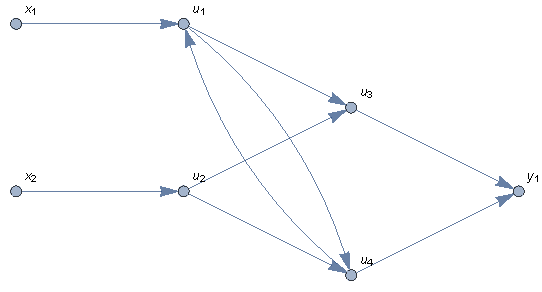
\includegraphics[width=3in]{DiGraph.pdf}
  \caption{Example Network}
  \label{fig:digraph}
\end{figure}
Which allows us to define the neural network as,
\begin{definition}
\normalfont A \textit{neural network} is a directed graph, $G$, where the vertices are redefined as \textit{neurons}, $V(G)=N(G)$, and edges redefined as \textit{connections}, $E(G)=C(G)$. The set $N(G)$ is partitioned into $N(G)=N_{in} \cup N_{out} \cup N_{hid}$, where $N_{in}\not =\emptyset$, $N_{out}\not = \emptyset$, and $N_{hid}\cap\left(N_{in}\cup N_{out}\right)=\emptyset$.

Where each connection, $uv$, carries a weight, $w_{uv}$, and each neuron, $u$, possesses four quantities: network input, $net_{u}$, activation, $act_{u}$, output, $out_{u}$, and external input, $ext_{u}$. Likewise, each neuron has three activation functions: $f^{u}_{net}:\mathbb{R}^{2\left\vert pred(u)\right\vert+\kappa_{1}(u)}\rightarrow \mathbb{R}$, $f^{u}_{act}:\mathbb{R}^{\kappa_2(u)}\rightarrow \mathbb{R}$, and $f^{u}_{out}:\mathbb{R}\rightarrow \mathbb{R}$, where $\kappa_{1}$ and $\kappa_{2}$ are dependent on the number of inputs.
\end{definition}
The \textit{adjacency matrix} or \textit{network structure} of $G$ is given as $M=\left\{w_{ij}\vert i,j\in [n(G)]\right\}$. If $G$ contains no self-loops or directed cyles, then $G$ is a \textit{feed forward} network, else $G$ is a \textit{recurrent} network.
\begin{figure}
$$\begin{array}{cccccccc}
  & x_1 & x_2 & u_1 & u_2 & u_3 & u_4 & y_1 \\
 x_1 & 0 & 0 & 2 & 0 & 0 & 0 & 0 \\
 x_2 & 0 & 0 & 0 & 2 & 0 & 0 & 0 \\
 u_1 & 0 & 0 & 0 & 0 & 4 & 0 & 0 \\
 u_2 & 0 & 0 & 0 & 0 & 3 & 3 & 0 \\
 u_3 & 0 & 0 & 0 & 0 & 0 & 0 & 1 \\
 u_4 & 0 & 0 & 2 & 0 & 0 & 0 & 0 \\
 y_1 & 0 & 0 & 0 & 0 & 0 & 0 & 0 \\
  \end{array}$$
  \caption{Example Network Structure}
 \end{figure}
\section{Digital Signal Processing and Sampling}
A near constant problem in the transmission of information is the inevitable presence of \textit{noise}. While a field of study in its own right, we utilize a few methods to aid in our signal processing~\cite{orfanidis_introduction_1996-1}~\cite{ulbikas_chaos_1998}~\cite{rodriguez-bermudez_analysis_2015}.
\subsection{Time Domain}
We receive data from the Cyton board roughly once a millisecond (as there can be a minor offset from system time to Cyton board time), the position of each node is given as,
$$\begin{array}{cccc}
  & \theta & r & \text{name}\\
1 & -39 & 0.333 & F3\\
2 & 0 & 0.256 & Fz\\
3 & 39 & 0.333 & F4\\
4 & -90 & 0.256 & C3\\
5 & 90 & 0 & Cz\\
6 & 90 & 0.256 & C4\\
7 & -141 & 0.33 & P3\\
8 & 141 & 0.333 & P4\\
\end{array}.$$ Eight channels give us row vectors of the form, $$f(t) = (x_1,x_2,x_3,x_4,x_5,x_6,x_7,x_8),$$
followed by the translation to phase space.
$$x_j=x(t+j\tau),$$
where $t$ is the start time, $\tau$ is our sampling rate, and $j$ is the channel index.
\subsection{Frequency Domain}
Utilizing the \textit{Discrete Fourier Transform} (DFT), $$F_n=\sum_{k=0}^{N-1}X_k  \cdot  e^{-2\pi i n k/N},$$
and \textit{Inverse Discrete Fourier Transform},
$$f_k=\frac{1}{N}\sum_{k}^{N-1}F_n\cdot e^{2\pi i n k/N},$$
we move between time and frequency domains. It's here that we utilize our digital filter, and claim multiplication in the frequency domain is equivalent to convolution in the time domain~\cite{orfanidis_introduction_1996-1}, and its complexity can be reduced from $O(n^2)$ to $O(n\log{n})$.
\begin{proof}
  \normalfont Let $f_1(t)$ and $f_2(t)$ be arbitrary vectors of $f(t)$. We define convolution as\\ $[f_1*f_2](t) = \sum_{v=-\infty}^{\infty}f_1(\tau)f_2(t-\tau)$\\
  $=\sum_{v=-\infty}^{\infty}f_1(t-\tau)f_2(\tau)$.\\
  This implies $[f_1*f_2](t) = \sum_{v=-\infty}^{\infty}f_1(\tau)f_2(t-\tau)$\\
  $=\sum_{v=-\infty}^{\infty}f_1(\tau)\sum_{v=-\infty}^{\infty}F_2(v)\cdot e^{2\pi i v(t-\tau)}$\\
  $=\sum_{v=-\infty}^{\infty}F_2(v)\sum_{v=-\infty}^{\infty}(f_1(\tau)\cdot e^{-2\pi i v\tau})e^{2\pi i v t}$,\\
  $=\sum_{v=\infty}^{\infty}F_{2}(v)F_{1}(v)e^{2\pi i v t}$,\\
  which is really,\\
  $=F_\tau^{-1}[F(\tau) F(\tau)](t)$\\
  and so by applying $F$ to both sides,
  $F[f_1*f_2]=F(f_2) F(f_1)$\\
\end{proof}
(For the non-discrete \href{http://mathworld.wolfram.com/ConvolutionTheorem.html}{convolution theorem})

\begin{figure}[ht]
  \centering
  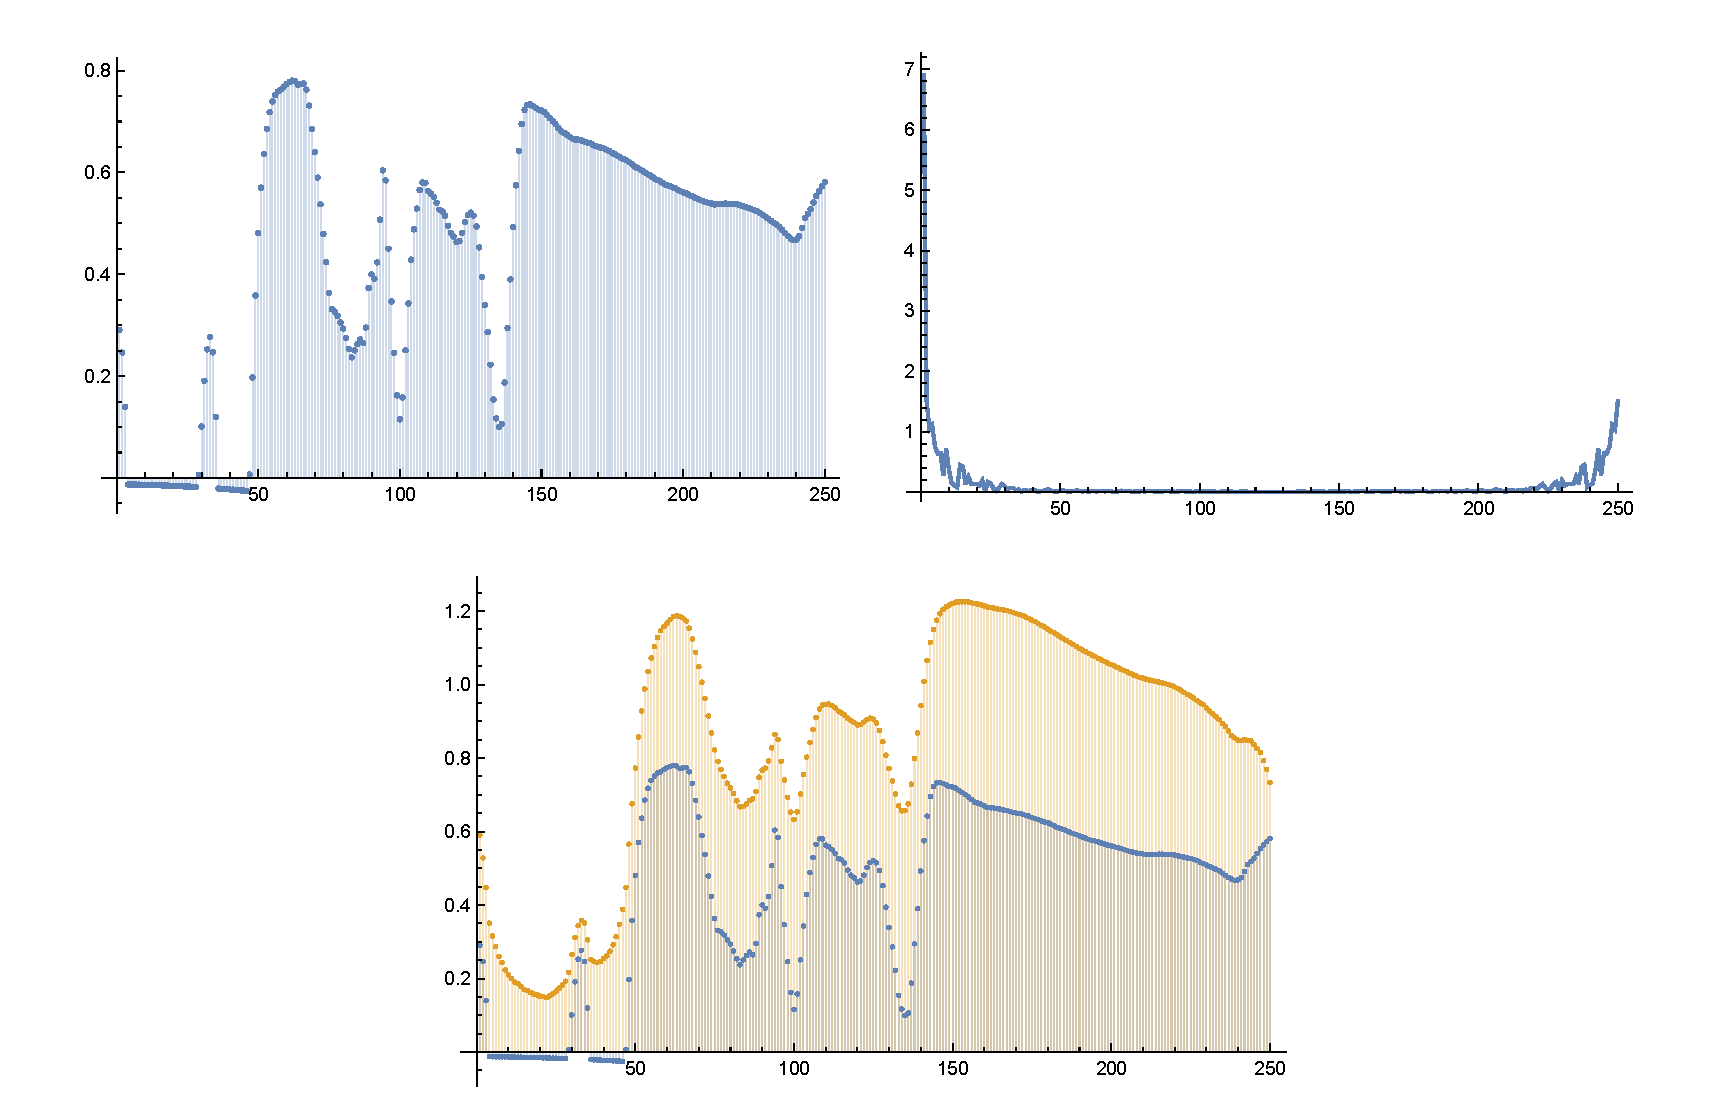
\includegraphics[width=4in]{Fourier.pdf}
  \caption{Top Left: Unfiltered data, Top Right: Translation to frequency domain, Bottom: Filter applied and translation back to the time domain}
  \label{fig:Fourier}
\end{figure}

Besides the benefit of more efficient filtering time, frequency information combined with the channel locations allows for some interesting visualizations~\ref{fig:HeadPlot}~\ref{fig:Freq}.

\begin{figure}[ht]
  \centering
  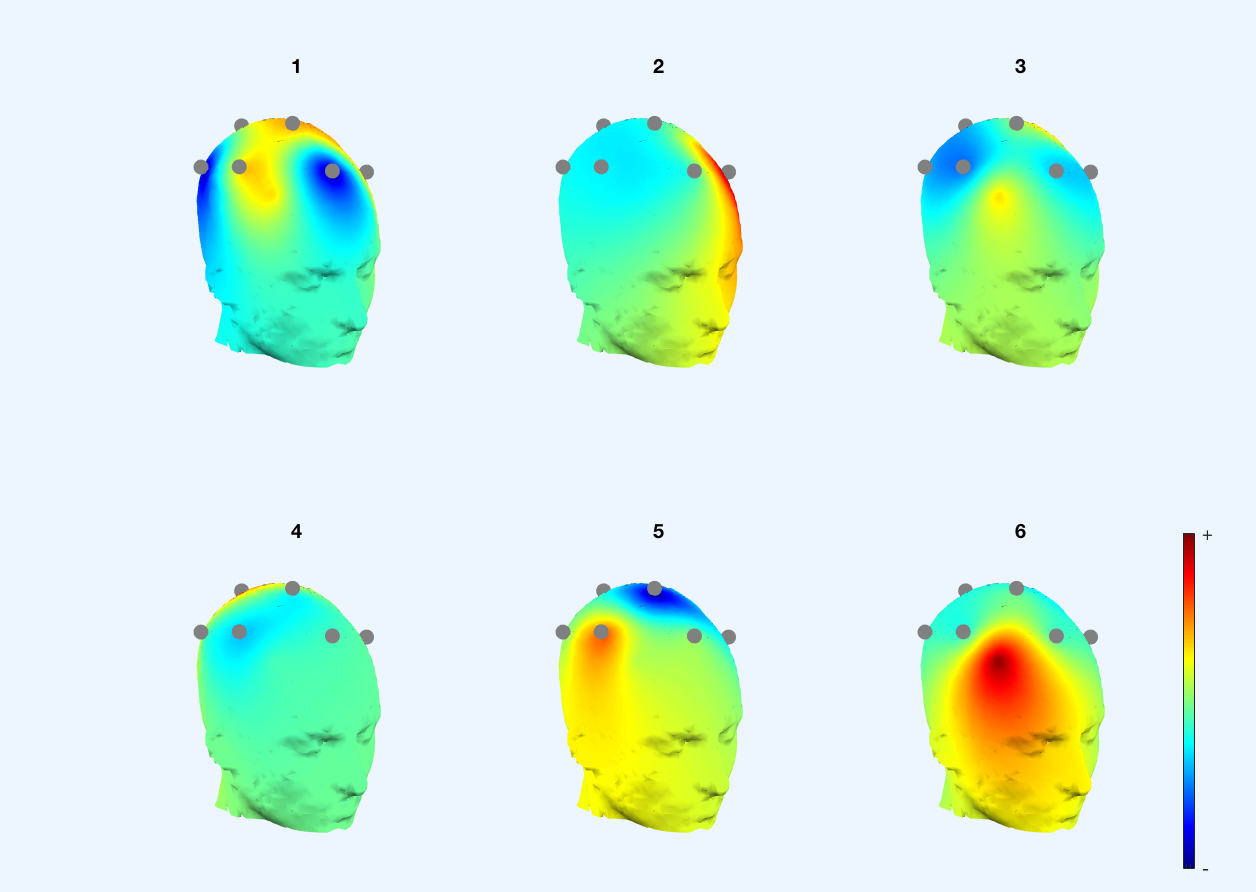
\includegraphics[width=2.5in]{HeadPlot.png}
  \caption{Head Plots showing activation}
  \label{fig:HeadPlot}
\end{figure}

\begin{figure}[ht]
  \centering
  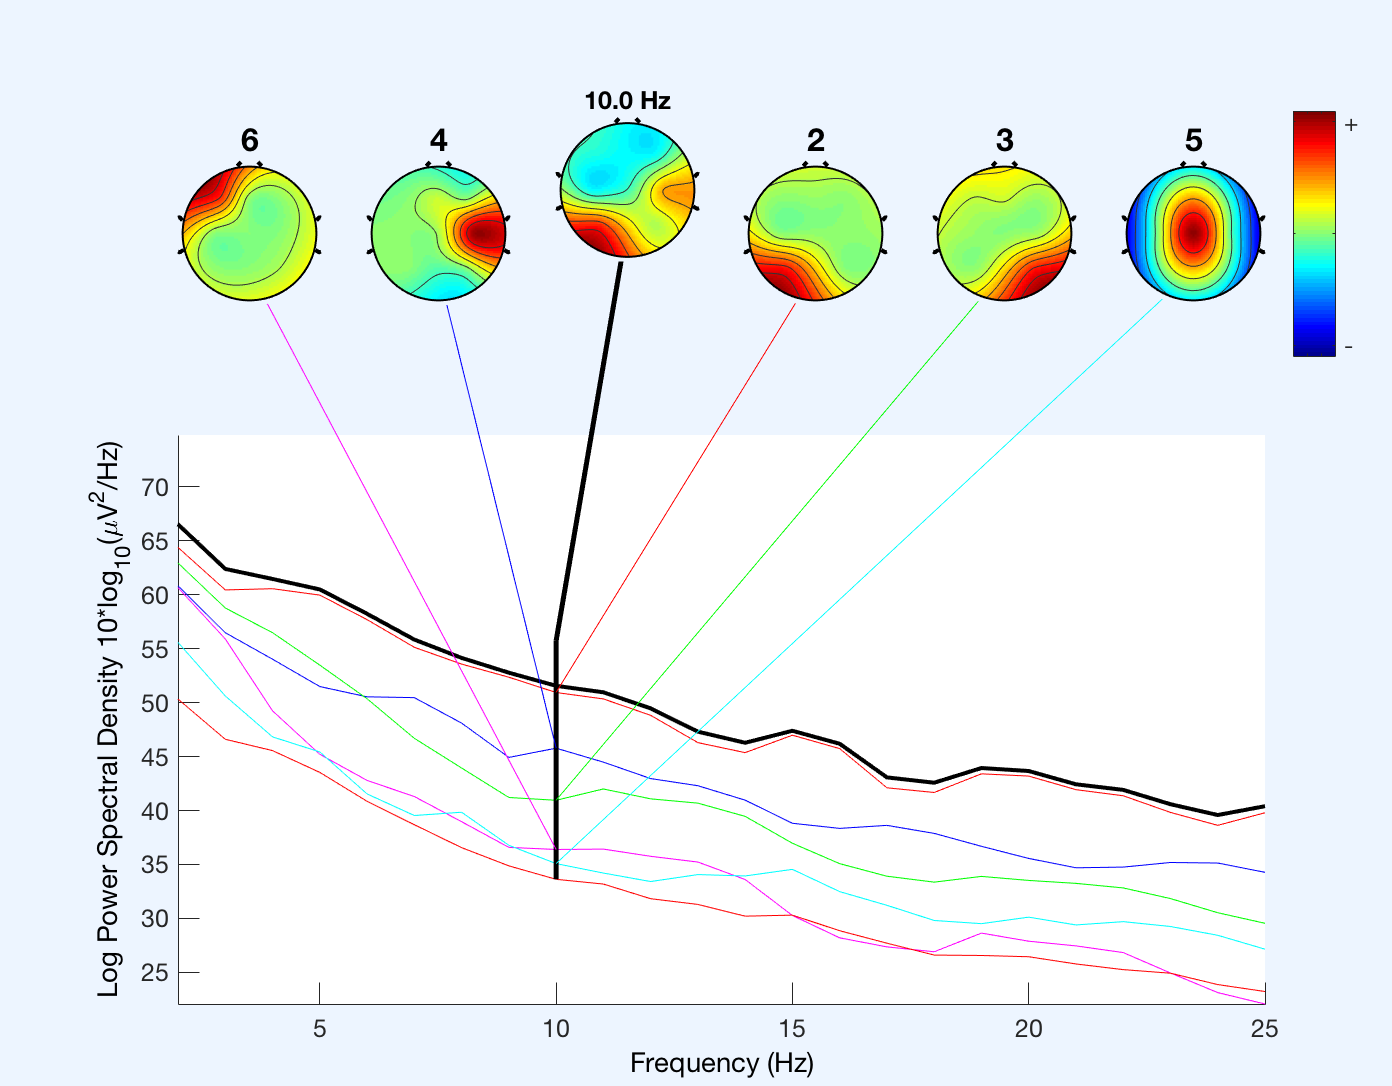
\includegraphics[width=2.5in]{Frequency.png}
  \caption{Map of six channels given a random 25\% of the data}
  \label{fig:Freq}
  \end{figure}
\subsection{Time-Frequency Domain}
While technically out of the scope of this project, a wavelet transform may be implemented in the future. This is due to more efficient computation time with regard to the DFT, as the computation of the Fourier matrix is $O(n\log{n})$~\cite{shwartz_ica_2004} whereas the Wavelet matrix is $O(n)$. The wavelet functions can be given as,
$$\psi^{a,b}(x)=\left\vert a\right\vert^{-1/2}\psi \left(\frac{x-b}{a}\right)$$
$$W_{\psi}(f)(a,b)=\frac{1}{\sqrt{a}}\int_{-\infty}^{\infty}f(t)\psi \left(\frac{t-b}{a}\right)d\,t,$$
for some $\psi(x)$, for example, the \href{http://mathworld.wolfram.com/HaarFunction.html}{Haar function},
$$\psi(x)=\begin{cases}
 -1 & \frac{1}{2}<x<1 \\
 1 & 0<x<\frac{1}{2} \\
 0 & \text{else}
\end{cases}.$$
Translation into the time-frequency domain affords us the ability to see potential activations at any one particular time interval. Of particular interest is the frequencies from $\SI{8}{\hertz}-\SI{12}{\hertz}$, or more commonly refered to as the \textit{alpha} band~\cite{czarnowski_patients_2018}.
\section{Artifact Rejection}
The presence of \textit{artifacts} in EEG data presents a serious problem for data interpretation. A leftover of transient electromyographic signals, fluctuations in the muscles beneath the scalp are interpreted and recorded by EEG devices. This produces a notable spike in both measured potentials as well as frequencies, which can be problematic when we're looking to define features of the given inputs.
\subsection{Preprocessing}
Following the recording of these data, we import (see Matlab subsection) to a toolbox where we can filter and run an \href{https://sccn.ucsd.edu/~jung/tutorial/runica.htm}{\textit{independent component analysis}}. This produces a maximally linearly independent set of vectors, which also smooths data spikes such as eye blinks~\cite{shwartz_ica_2004}.

Now that we have filtered data with minimal artifacts, we can start to consider our computational intelligence approach. Features will be found in these newly processed data sets, all that remains is to convert them to a json file format for use by our neural network. However, it's necessary to train the given network given a set of inputs and expected outputs. The implication then is that we must design an experimentation framework to record different expected outputs.

Once this is achieved, we can begin to train two ANNs against both processed and unprocessed data. The first network must be trained to extract artifacts, and return data similar to the processed data, and the second must analyze said processed data and make predictions regarding future input. Both processes must also have a predecessor data filter.

We're currently training a \textit{Nonlinear Autoregressive Exogenous} model to accurately predict and respond to blinks, simply for our own edification~\cite{xiu_multivariate_nodate}.

\begin{figure}[ht]
  \centering
  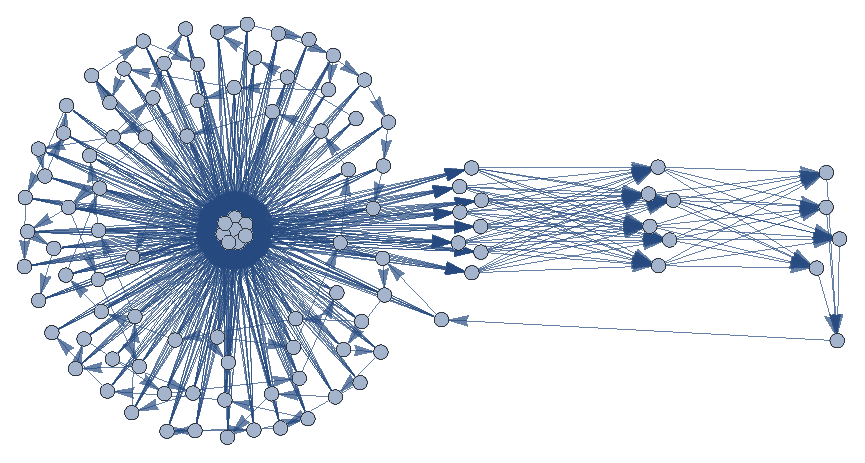
\includegraphics[width=4in]{narx.pdf}
  \caption{Our NARX}
  \label{fig:narx}
\end{figure}

\begin{figure}[ht]
  \centering
  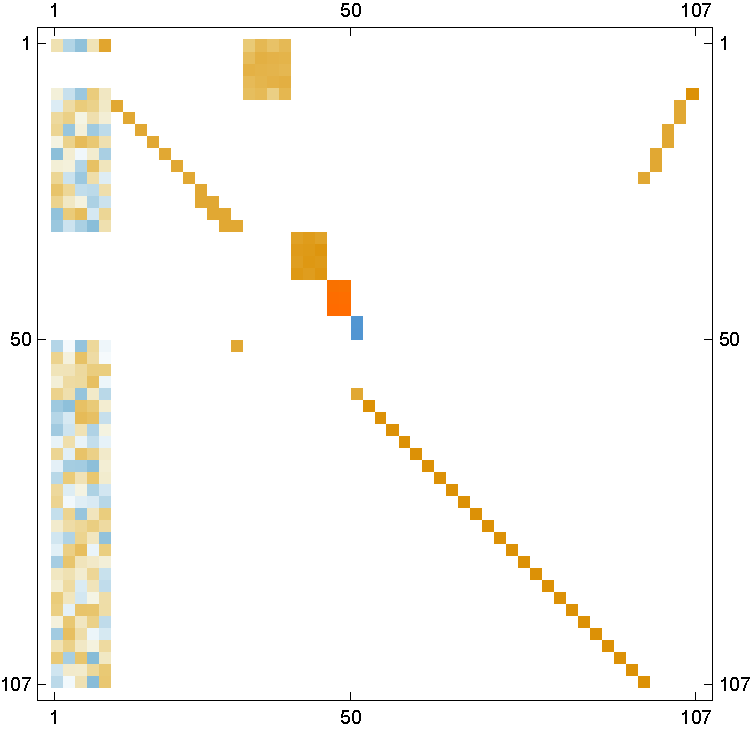
\includegraphics[width=2in]{networkstruc.pdf}
  \caption{Network Structure}
  \label{fig:netstruc}
\end{figure}

\section{Implementations}
For the current project code, please see \href{https://github.com/mahn00b/openbci_testing_e}{this repository}. We're currently working to establish a database, using MongoDB, for the storage of EEG data. Being as these data can be sensitive, we also intend to implement safe storage procedures to secure the privacy of any volunteers helping us collect data.
\subsection{Matlab/Octave}
This function was written to automate the preprocessing of recorded data using the OpenBCI GUI. It applies the necessary filters, followed by the independent component analysis, before outputing the data as a set file. These data must be converted back to micro volts before the ANN is trained, as well as converted to the appropriate json format.
\lstinputlisting[language=Matlab
  ,caption=Matlab/Octave Dataset Function]{OpenBCIDATA.m}
%%%%%%%%%%%%%%%%%%%%%%%%%%%%%%
% Uncomment region for Node.js code
%% \subsection{Node.js}
%% Both of the following files were adapted from \href{https://github.com/NeuroJS/openbci-experimenter}{experimenter} and \href{https://github.com/NeuroJS/openbci-neural-trainer}{trainer} respectively. We'd like to thank Alex Castillo for making these repositories public. Likewise, our ANN implementations would not be possible if not for \href{https://wagenaartje.github.io/neataptic/}{neataptic}, \href{https://github.com/NeuroJS/synaptic}{synaptic}, and \href{https://github.com/OpenBCI/OpenBCI_NodeJS}{OpenBCI SDK}.
%% \lstinputlisting[language=JavaScript,caption=Node.js Experimenter]{experiment.js}

%% \lstinputlisting[language=JavaScript,caption=Node.js Neural Net Trainer]{trainer.js}

\section{Proposal for Future Work}
The developing field of robotics/bionics promises to provide affordable, customized prosthetic equipment to those in need. We'd like to formally request the following materials in order to contribute what we can. A link to the project website can be found \href{https://hackaday.io/project/4745-openbionics-affordable-prosthetic-hands#menu-description}{here}.\\
- 1 x \href{http://www.dfrobot.com/index.php?route=product/product&product_id=964#.Vi075rfhDIU}{servo}\\
- 1  x \href{http://www.ebay.com/itm/Super-Strong-PE-Dyneema-Spectra-Extreme-Braid-Fishing-Line-300M-50LB-0-4mm-Green-/231522434670?hash=item35e7cffe6e:m:mS6JDkM3QDWhsCaMIFI_EGA}{dyneema fishing line}\\
- 1 x \href{http://www.amazon.com/gp/product/B00MUBWYL0?keywords=nylon%20fishing%20line%200.4&qid=1445805110&ref_=sr_1_6&sr=8-6}{nylon fishing line}\\
- 1 x \href{http://www.ebay.com/itm/20-PCS-3x12x4mm-1-2mm-Deep-V-Groove-Sealed-Guide-Pulley-Rail-Ball-Bearing-623VV-/171383515745}{pulleys}\\
- 1 x \href{http://www.amazon.com/Frost-King-R338H-Sponge-16-Inch/dp/B000BQWWF4/ref=sr_1_1?ie=UTF8&qid=1445803937&sr=8-1&keywords=sponge+tape+3%2F8+3%2F16}{sponge tape}\\
- 1 x \href{http://www.amazon.com/Scotch-23-Electrical-Width-Length/dp/B000V4P58M/ref=sr_1_1?ie=UTF8&qid=1445804020&sr=8-1&keywords=rubber+tape+scotch+23}{adhesive-tape}\\
- 1 x \href{http://www.vikingtapes.co.uk/p-1713-safety-grip-self-adhesive-tape-25mm-x-183m.aspx#.Vi085bfhDIV}{safety grip tape}\\
- 1 x \href{http://www.homedepot.com/p/VELCRO-brand-5-ft-x-3-4-in-Sticky-Back-Tape-90086/202261917}{velcro}\\
- 1 x \href{http://www.homedepot.com/p/Waddell-3-4-in-x-72-in-Hardwood-Round-Dowel-6440U/204397063}{wooden dowel}\\
- 1 x \href{http://www.amazon.com/gp/product/B008EQ1KJW?psc=1&redirect=true&ref_=oh_aui_detailpage_o00_s00}{arm sleeve}\\
- 1 x 4mm silicone sheet\\
- 1 x 5mm silicone sheet\\
In addition, we'd like to request ready access to a 3D-printer along with,\\
- 1 x \href{https://www.amazon.com/dp/B014KVDXUS/ref=twister_B01LXZYJ3R?_encoding=UTF8&psc=1}{NinjaFlex TPU filament}\\
- 1 x \href{https://www.matterhackers.com/store/l/black-pro-series-abs-filament-175mm-1kg/sk/M6A3VYQ9}{MatterHackers ABS filament}\\
And finally, the following from OpenBCI,\\
- 1 x \href{https://shop.openbci.com/collections/frontpage/products/wifi-shield?variant=44534009550}{wifi-shield}\\
- 1 x \href{https://shop.openbci.com/collections/frontpage/products/myoware-muscle-sensor?variant=29472011267}{Myoware-muscle-sensor}\\
- 1 x \href{https://shop.openbci.com/collections/frontpage/products/pulse-sensor}{pulse-sensor}\\
- 1 x \href{https://shop.openbci.com/collections/frontpage/products/cyton-daisy-biosensing-boards-16-channel?variant=38959256526}{Cyton-Daisy Biosensing board}\\
%\newpage
%\section{References}

\bibliography{Modeling.bib}
\bibliographystyle{plain}
\end{document}
